\section{Conclusion}
In this chapter, we have presented a background of current approaches that deal with the integration of heterogeneous models and languages, in both a structural and a behavioral way. 

We have presented approaches the combine structural models/languages in order to obtain a new model/language. 

To compose models, some of these approaches consider syntactical similarities between models, whereas others take also into account the behavior of models. 

We have determined that these approaches only compose homogeneous models.    

Similarly, to compose languages, some of these approach only consider the syntax whereas others also considers both the sinyax and the semantics in order to get a composed language. 

 

Afterwards, we have presented the state of art approaches that deal with coordination of the behavior of models/languages. 





 Conversely, we have presented the work done by Coordination Languages and ADLs that support the coordination of heterogeneous models. However, the system designer has to manually specify each relation, thus making this task tedious and error prone.
 
 Then, we have shown how coordination pattern approaches have leveraged on the know-how of system designer to automate the coordination between models.
 
 However, we have noted that the knowledge about system integration is encoded within a framework. 
 
 Furthermore, in frameworks, the model of coordination is expressed by using a general purpose language thus limiting verification and validation activities. 

To capture explicitly the know-how of a system designer, we propose \bcool a dedicated language to capture coordination patterns between languages, thus reifying coordination at the language level (see Figure~\ref{fig:bcoolapp}). From this specification, a formal model of coordination is generated. 


This enables validation and verification of the coordinated system. 


In the next chapter, we focus on coordination pattern approaches to understand how a coordination pattern is being captured. We leverage on such knowledge to build \bcool. 

\begin{figure}
\begin{center}
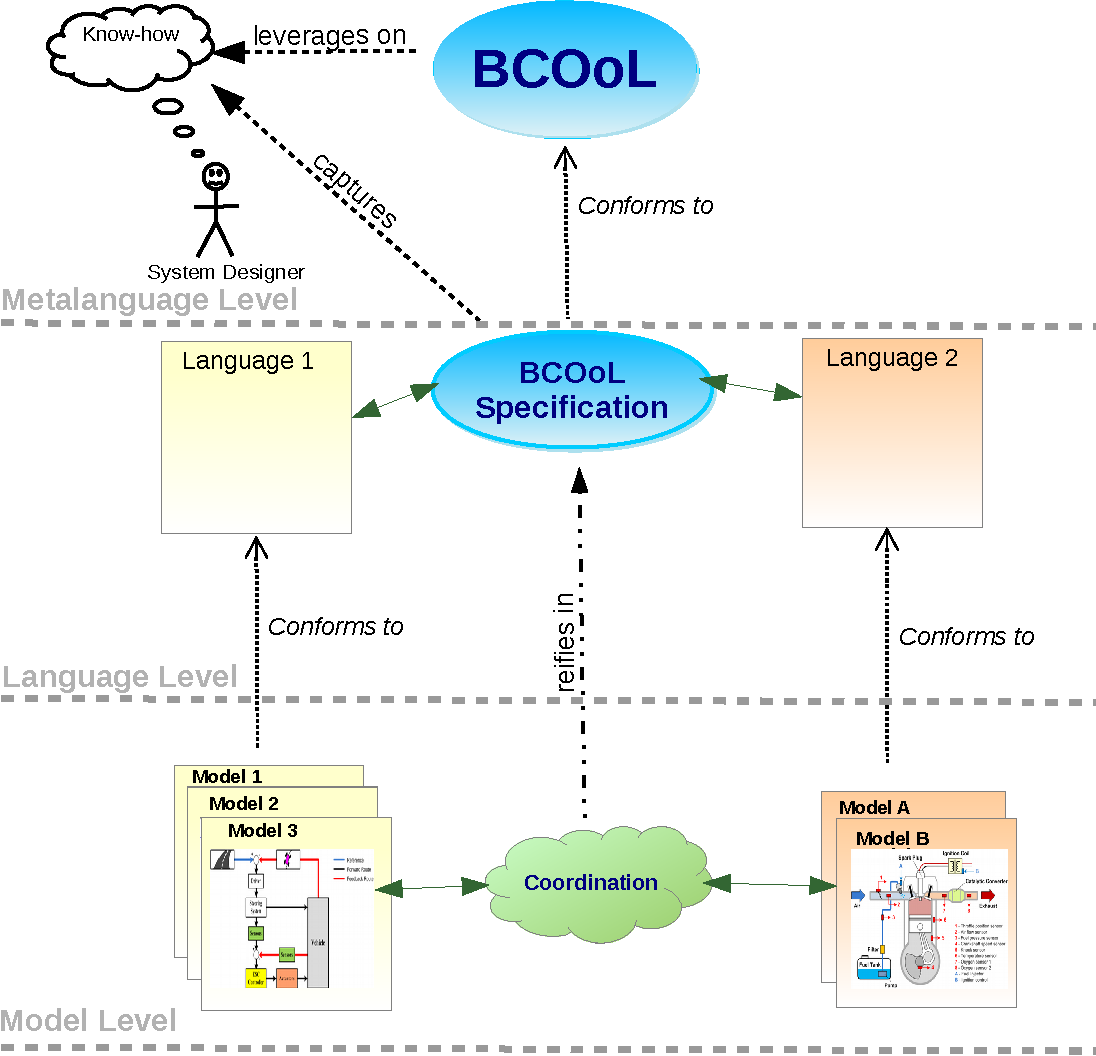
\includegraphics[width=0.7\textwidth]{background/figs/bcoolapp}
\caption{Overview of Our Approach}
\label{fig:bcoolapp}
\end{center}
\end{figure}	


%\begin{landscape}% Landscape page
%\begin{table}[]
	%\centering
	%\caption{Overview of Behavioral Composition/Coordination Approaches}
	%\label{tbl:overview}
	%\resizebox{\textwidth}{!}{%
		%\begin{tabular}{@{}|c|l|l|c|c|c|c|c|c|c|
			%	>{\columncolor[HTML]{9AFF99}}c |@{}}
			%\toprule
			%\multicolumn{3}{|c|}{} & \multicolumn{2}{c|}{Behavioral Composition Approaches} & \multicolumn{3}{c|}{Coordination %of Model Approaches} & \multicolumn{2}{c|}{Coordination Pattern Approaches} & Our Approach \\ \cmidrule(l){4-11} 
			%\multicolumn{3}{|c|}{\multirow{-2}{*}{}} & Semantic Anchoring & \cite{compostatechartsbib} & Esper & Rapide & BIP & %Ptolemy & Di Natale et. al & BCOoL \\ \midrule
			%\multicolumn{3}{|c|}{Number of Languages/Models Supported} & 1 & 1 & N & N & 1 & Predefined set & 2 & N Languages %\\ \midrule
			%\multicolumn{3}{|c|}{Specification of the Coordination (from a system designer point of view)} &  & Implicit & %Explicit & Explicit & Explicit & Implicit & Impicit & Explicit \\ \midrule
			%\multicolumn{3}{|c|}{Glue (coordination at model level)} &  &  & Formal & Formal & Formal & Java (generated) & C++ %(generated) & Formal (generated) \\ \bottomrule
%		\end{tabular}
%	}
%\end{table}
%\end{landscape}
